\subsection{Task 5.3 -- Continuous Delivery/Deployment}

Workflow \nolinkurl{.github/workflows/cd.yml} tự chạy khi có push vào
\texttt{main}, bao gồm commit sau khi merge PR. Workflow cũng hỗ trợ tag
\nolinkurl{v*} và chạy thủ công. Các bước phát hành chạy theo thứ tự sau.

\begin{enumerate}[leftmargin=*]
  \item \textbf{Quality gate.} Gọi lại CI trên cùng commit để chạy lint,
        unit test, build, kiểm thử tích hợp và E2E. Chỉ chuyển sang đóng gói
        khi toàn bộ job kiểm tra đạt.
  \item \textbf{Đóng gói.} Build hai Docker image web và API, gắn tag bằng
        commit SHA và đẩy lên GitHub Container Registry.
  \item \textbf{Kiểm tra đích và migration.} Dùng secrets từ GitHub
        Environment \texttt{production}. Kiểm tra đích Render/Vercel và xác
        nhận baseline migration cùng bản sao lưu. Sau đó chạy
        \texttt{prisma migrate deploy} trên Supabase.
  \item \textbf{Deploy và smoke test.} Render triển khai API từ SHA phát hành.
        Vercel CLI triển khai web từ cùng checkout. Workflow kiểm tra
        \nolinkurl{/api/health}, \nolinkurl{/api/products}, trang web HTTPS và
        health endpoint qua proxy web. Image GHCR lưu bản đóng gói theo SHA
        để truy vết.
\end{enumerate}

Nếu rollout lỗi sau khi đã cập nhật một ứng dụng, workflow thử khôi phục bản
Vercel trước đó hoặc commit Render trước đó, tùy bước đã thành công. Rollback
schema và dữ liệu PostgreSQL được xử lý riêng theo
\nolinkurl{docs/deployment.md}.
\href{https://github.com/PhucTruong11/brewlite-assignment2/actions/runs/43554939814}{Lượt phát hành của commit \texttt{c3e9ae3}}
ghi nhận CI, publish image, migration, deploy và smoke test đều đạt.

\paragraph{Minh chứng phát hành ngày 19/11/2026}
Ảnh nhóm cung cấp ghi nhận lượt CD \#14 sau khi merge PR \#10 vào
\texttt{main}, tại commit \texttt{9e35333}. Trạng thái tổng thể là
\texttt{Success}, thời gian 6 phút 49 giây. Ba giai đoạn CI trước release,
build/publish image theo SHA và migrate/deploy/smoke test đều đạt.

\begin{reportfigure}
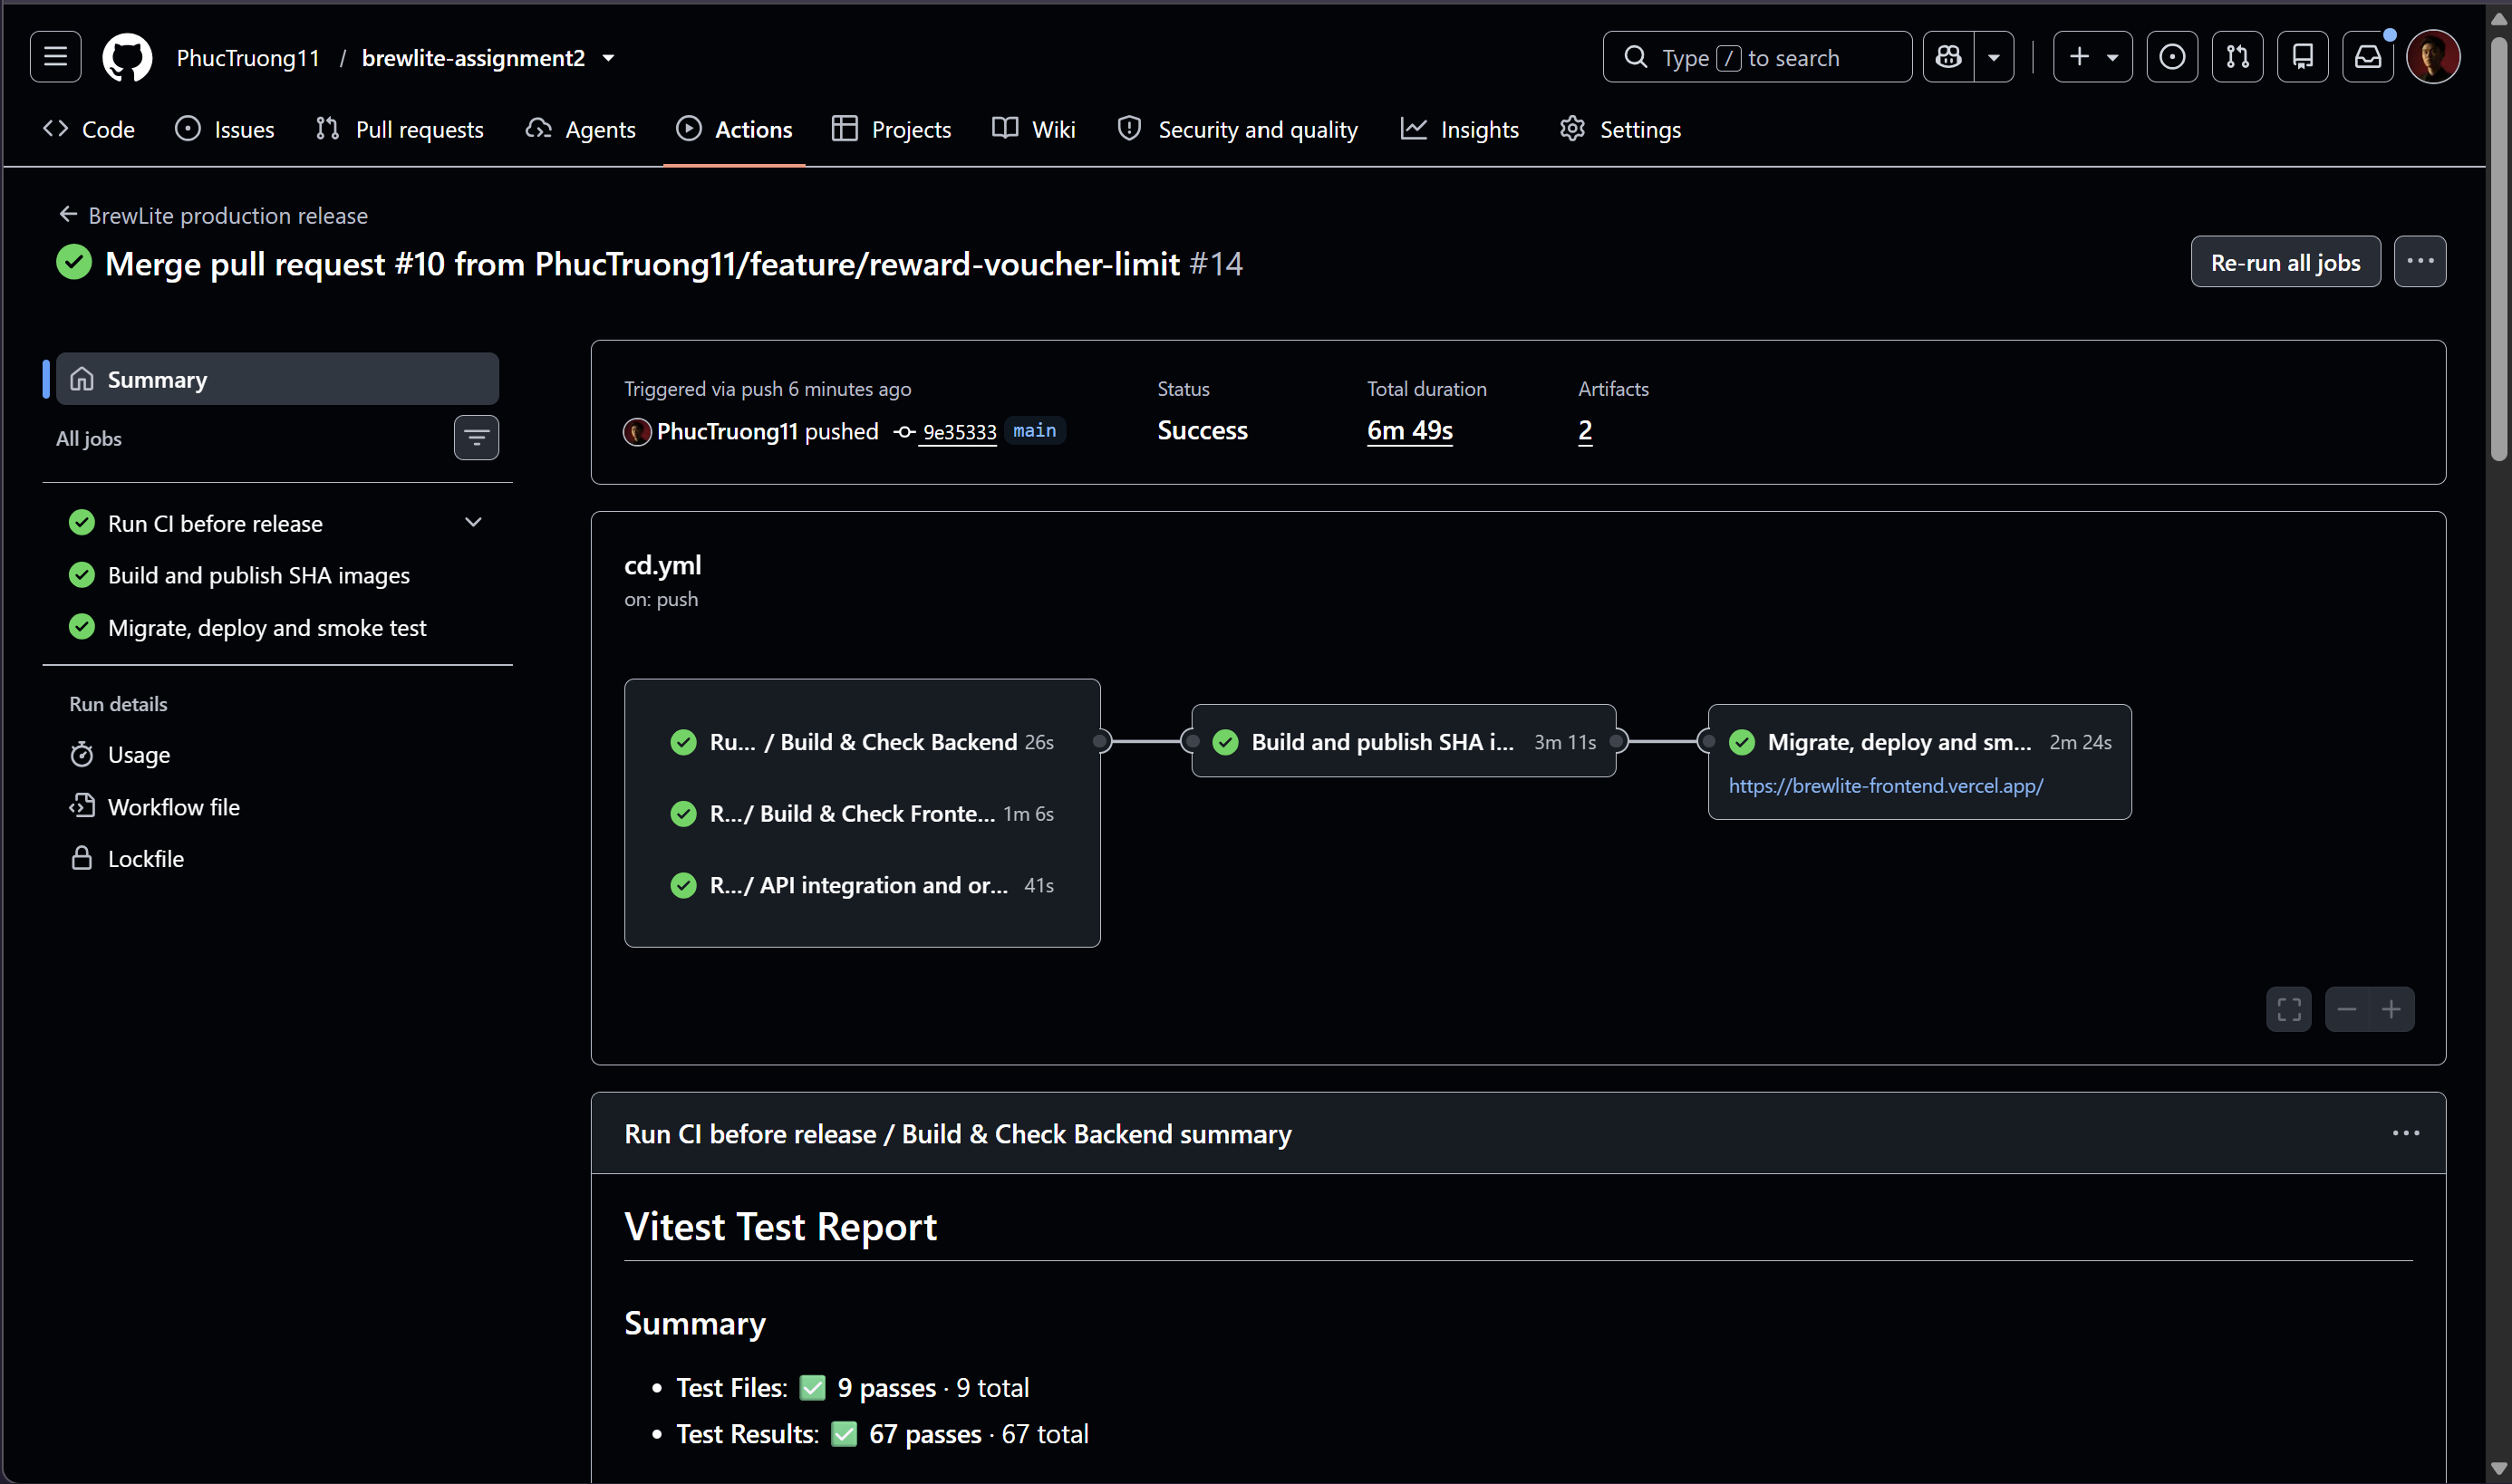
\includegraphics[width=\linewidth,trim=0bp 185bp 0bp 65bp,clip]{../../assets/evidence/cd-success.png}
\par\small\itshape Hình 5.3a. CD thành công: CI $\rightarrow$ image theo SHA
$\rightarrow$ migration, deploy và smoke test
\end{reportfigure}

Ảnh Render ở Hình 5.3c hiển thị cùng commit \texttt{9e35333} ở trạng thái
\texttt{Live}. Ảnh Vercel ở Hình 5.3b hiển thị deployment production
\texttt{Ready} từ \texttt{main} với nội dung merge PR \#10. Các ảnh này
đối chiếu kết quả workflow với trạng thái dịch vụ tại thời điểm chụp.

\paragraph{Web production trên Vercel}
Ảnh nhóm cung cấp ngày 19/11/2026 hiển thị deployment ở trạng thái
\texttt{Ready}, môi trường \texttt{Production -- Current}, nguồn
\texttt{main} và nội dung merge PR \#10. Domain production là
\nolinkurl{brewlite-frontend.vercel.app}.

\begin{reportfigure}
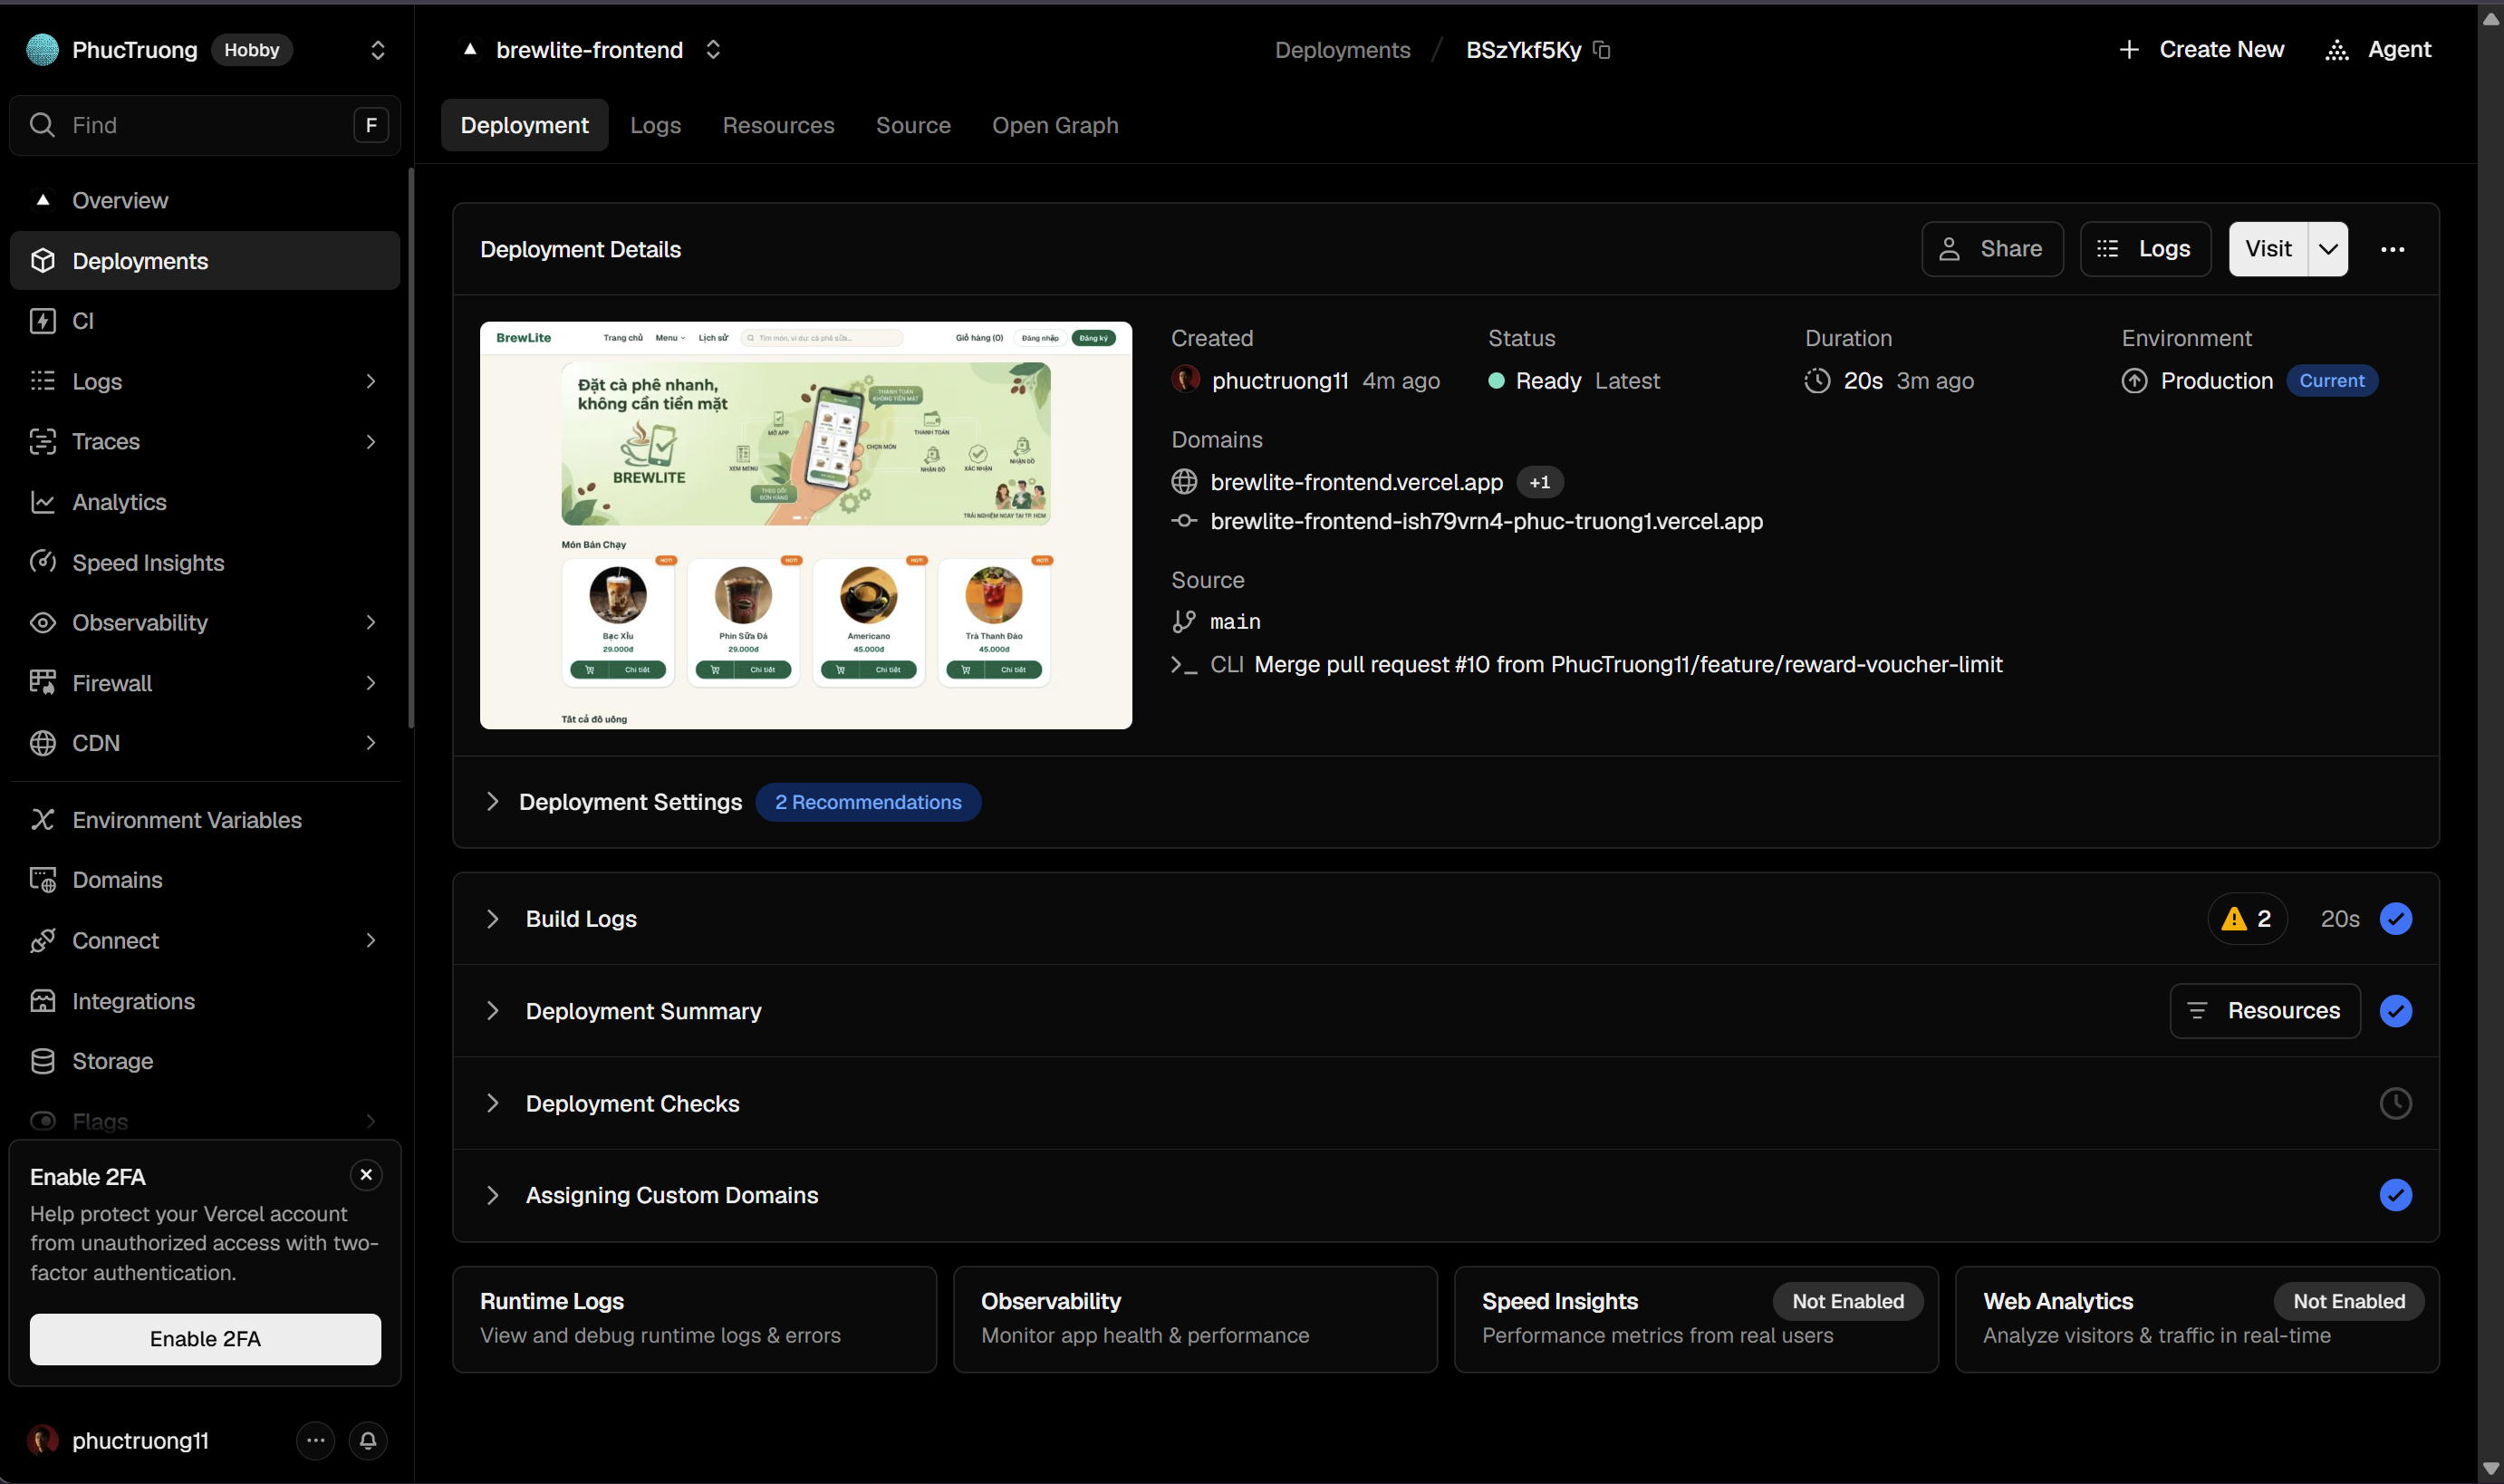
\includegraphics[width=\linewidth,trim=475bp 310bp 30bp 130bp,clip]{../../assets/evidence/vercel-ready.png}
\par\small\itshape Hình 5.3b. Deployment frontend production trên Vercel
\end{reportfigure}

Ảnh giao diện truy cập được từ domain này nằm ở Hình 4.3a--4.3c.
Trạng thái \texttt{Ready} trong dashboard là minh chứng triển khai tại thời
điểm chụp; kết quả smoke test được đối chiếu ở Hình 5.3a.

\paragraph{API production trên Render}\leavevmode\par\nobreak
\begin{reportfigure}
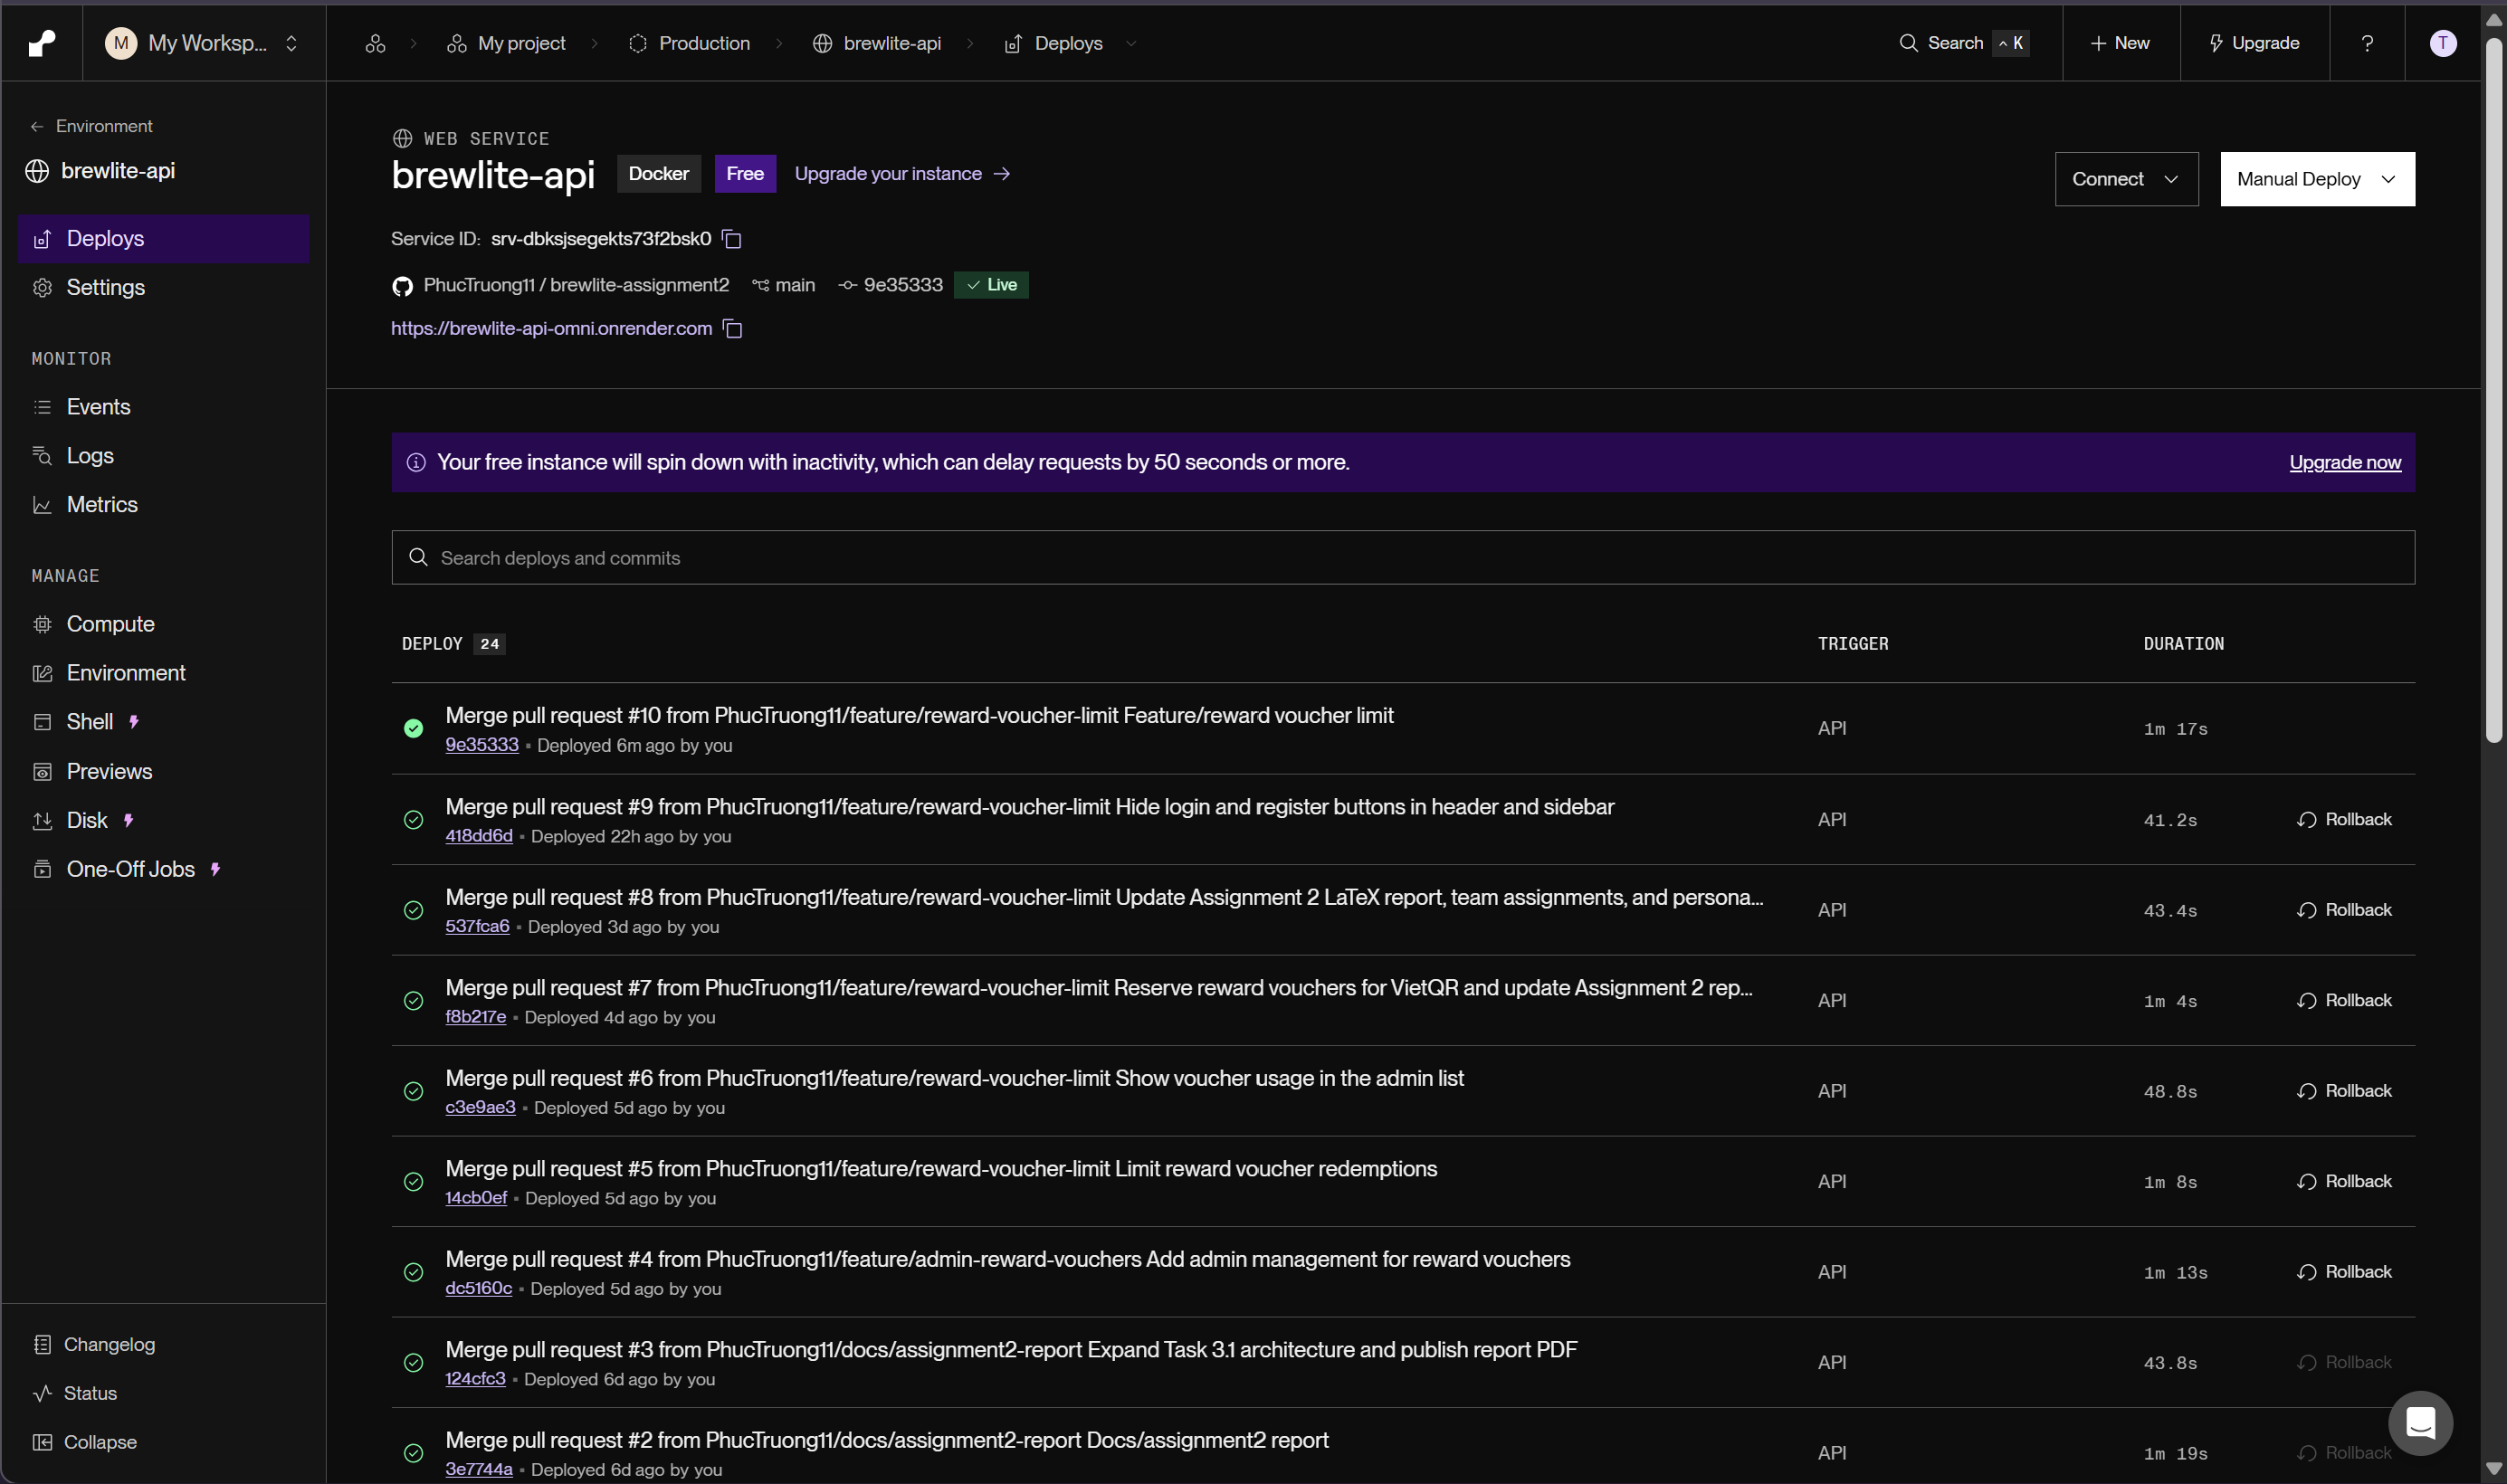
\includegraphics[width=.85\linewidth,trim=157bp 450bp 490bp 40bp,clip]{../../assets/evidence/render-live.png}
\par\small\itshape Hình 5.3c. API Render ở trạng thái Live, commit 9e35333
\end{reportfigure}

Render hiển thị repository \nolinkurl{PhucTruong11/brewlite-assignment2},
nhánh \texttt{main} và endpoint \nolinkurl{brewlite-api-omni.onrender.com}.
Đây là cùng SHA trong minh chứng CD tại Task 5.3.

\paragraph{PostgreSQL production trên Supabase}\leavevmode\par\nobreak
\begin{reportfigure}
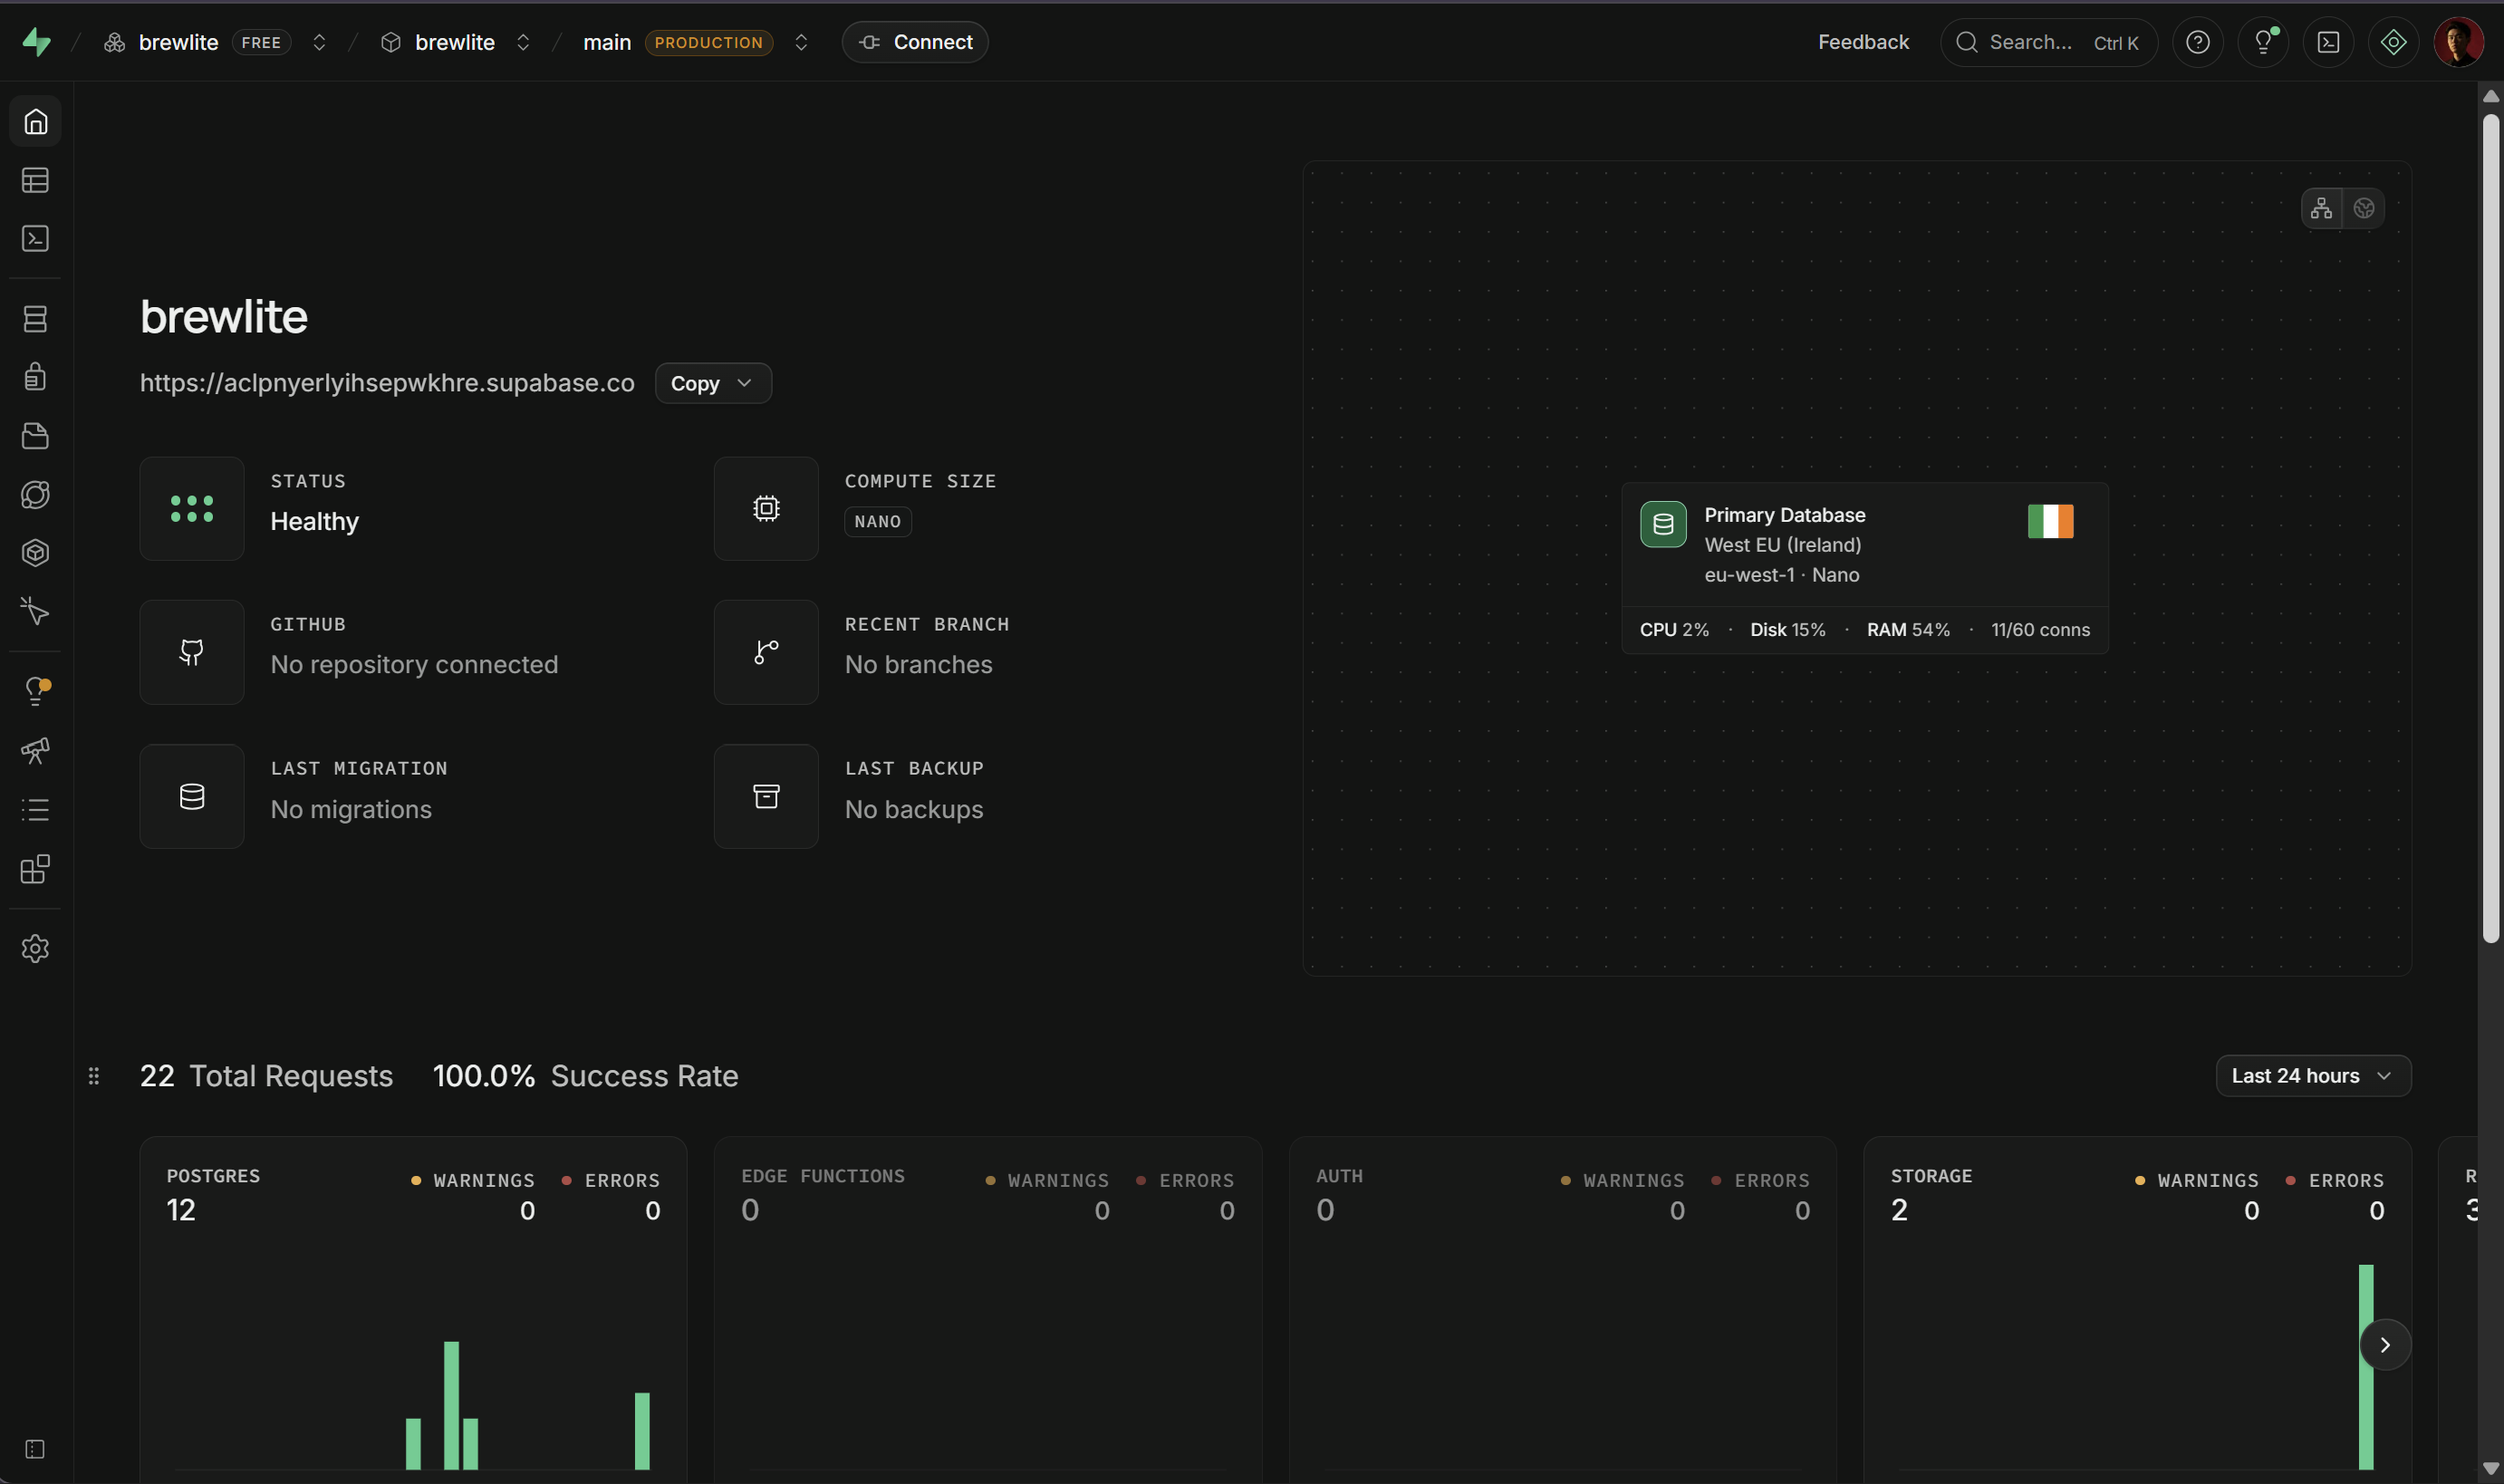
\includegraphics[width=\linewidth,trim=40bp 235bp 30bp 0bp,clip]{../../assets/evidence/supabase-healthy.png}
\par\small\itshape Hình 5.3d. Dự án Supabase Healthy và Primary Database tại thời điểm chụp
\end{reportfigure}

Dashboard hiển thị dự án ở trạng thái \texttt{Healthy}, DB Nano tại vùng
\texttt{eu-west-1} (Ireland). Đây là dịch vụ PostgreSQL production mà API
Render sử dụng để lưu dữ liệu nghiệp vụ.
